\documentclass[journal,12pt,onecolumn]{IEEEtran}
\usepackage{amsmath}
\usepackage{amssymb}
\usepackage{enumerate}
\usepackage[utf8]{inputenc}
\usepackage{multicol}
\usepackage{gensymb}
\usepackage{nopageno}
\usepackage{mathtools}
\usepackage{siunitx}
\usepackage{graphicx}
\DeclareUnicodeCharacter{2212}{-}
\graphicspath{{/home/diparna/Documents/WORK_ADP/AdaptiveSignal Processing 7}}
\begin{document}
\centering \textbf{EE608  Adaptive Signal Processing}\\
\medskip
\centering{Problem Set 7}\\
\medskip
\begin{enumerate}
\item As shown in class the decision feedback equalizer is obtained by finding $\alpha_k $ and $ \beta_k$ such that\\
$E[{\mid{I_k}-{\hat{I}_k}\mid}^2]$ is minimized\\
\bigskip
subject to
$${\hat{I}}_k=\sum_{k={-M_1}}^0{\alpha_k}y(k-n)+\sum_{k=1}^{M_2}{\beta_k}{I_{k-n}}$$\\
\bigskip
Show that $\{\alpha_k,\beta_k\}$ are obtained by solving\\
\medskip
$$\sum_{j=-{M_1}}^{0}{\alpha_j}r(l_1-j)+\sum_{j=1}^{M_2}{\beta_j}q^*(j-l_1)=q^*(-l_1)$$\\
\bigskip
$$\sum_{j=-{M_1}}^{0}{\alpha_j}q(-j+l_2)1(L+j-l_2)+\beta_{l_2}=0$$\\
\bigskip
where $M_1\leq {l_1}\leq 0$ and $1\leq{l_1}\leq M_2.$\\
In the above $q(\cdot)$ is the impulse response sequence such that the preprocessed received signal (preprocessed in the
sense that the received signal has gone through a matched filter and a whitening filter) is given by\\
\medskip
$$y(k)= \quad\sum_{n=0}^{L}q(n)I_{k-n}+\eta(k)$$\\
\bigskip
where we assume that $I_n \perp\!\!\!\perp $ $I_m$ for $m \neq n,$ and $E[I_nI_m^{*}]=\delta_{m,n}.$ Also $I_n \perp\!\!\!\perp \eta(k)$ for all n and k, and $E_\eta(k)\eta(l)=\sigma_n\delta_{k,l}.$   
\medskip
\item Derive the update equation for the the training based LMS Algorithm for adaptive equalization, namely\\
\bigskip
$W(n+1)=W(n)+\mu {Y^*(n)}[I(n)-Y^T(n)W(n)],W(0)=0$\\
\medskip
\item Derive the CM algorithm of Goddard for the case for\\
\medskip
$J_{12}={(\vert\hat{I}_k\vert -D)}^2$\\
Derive the weight update equation as well as the carrier tracking equation.\\
\textbf{Simulations}
\item \textbf{LMS algorithm for channel equalization using training signals:}\\
Consider the following block diagram for the adaptive channel equalizer using training sequences.\\
\bigskip
\bigskip
In the above we are assuming that the transmitted symbols are binary (bpsk) with zero mean $b_n=\pm 1$. These are passed through a channel with impulse response\\
\medskip
$h(n)=\begin{cases}
\frac{1}{2}[1+cos(\frac{2\pi}{F}{(n-2)})]& n=1,2,3\\
0 & otherwise
\end{cases}$\\
\medskip
\begin{center}
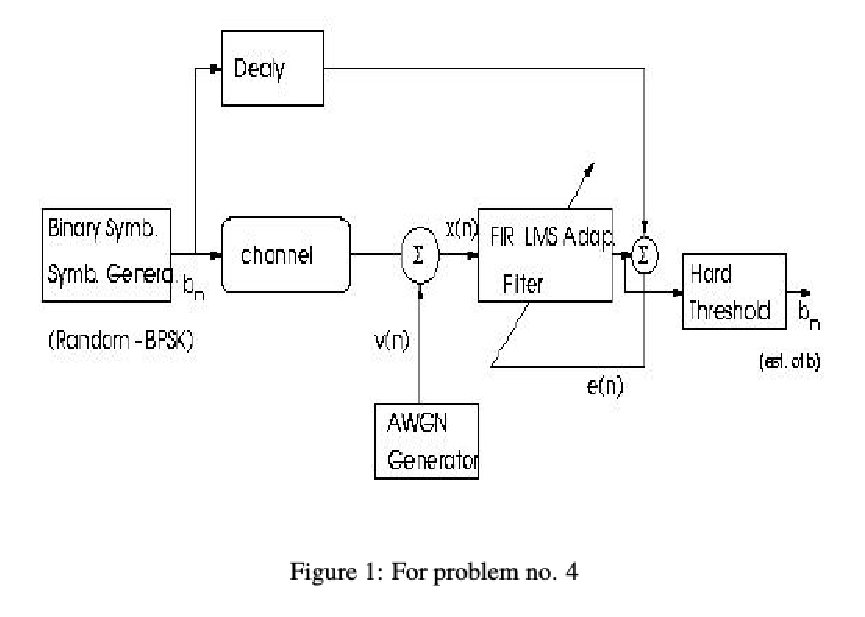
\includegraphics[scale=.8]{figure3.eps}\\
\end{center}
\smallskip
and corrupted by additive white Gaussian noise (AWGN) with zero mean and variance $\sigma^2$. The delayed symbols that are fed at the output of the adaptive filter act as training signals.The channel impulse response is an 3-point FIR filter with a raised cosine type of structure.Parameter F controls the eigen value spread of $R=E[X(n)X^T(n)$.The structure of this problem is very similar to the one given in Haykin.\\
\medskip
Note:\\ 
\medskip
$$x(n)=\quad\sum_{k=1}^{3}h(k)b_{n-k}+v(n)$$\\
\medskip
You will need two random number generators; one for the symbols b n and the other for the AWGN.For AWGN assume $\sigma^2=0.01.$ For $b_n$ use a binary random number generator where 1 and -1 are generated with equal probability. You could do this by using a uniform random number generator, uniform over [−0.5, 0.5]. Whenever you get a negative number, set it to -1 and whenever you get a positive number set it to +1.
\medskip
\begin{enumerate}[(a)]
\item Experiment with different number of tap weights in the FIR LMS adaptive filter. For example you could consider 7, 9, or 11 tap weights.
\item Experiment with different variance for AWGN.
\item Estimate the amount of delay you need based on the number of tap weights you are using.
\item Run the experiment for two vales of $F$, say $F=3$ and $F=3.2$.
\item Plot the mean square error curves for each case.
\item Give a table for the values for $W(\infty).$
\item At the output of the adaptive filter have a hard threshold unit to classify the output as 1 or -1. This is done since we know that the transmitted symbols were 1 or -1. Now compute the percentage bits that are in error at convergence (this will give you the bit error rate (BER)).
\end{enumerate}
\medskip
\item Repeat the above channel equalization problem for the following cases:
\medskip
\begin{enumerate}[(a)]
\item The channel is no longer as given by the cosine function. But, now let the channel be modeled by an FIR filter of length 10, and each FIR coefficient be of unit magnitude. This way we will be considering the performance of the equalizer under a narrow band channel.
\item The data symbols are not binary (BPSK) but are QPSK. You can generalize the method used for generating BPSK to a method for generating QPSK. Plot the bit error rate. Do this for both the cases: (a) the FIR channel specified above, and (b) any other narrow band channel of your choice. Your channel could be FIR, IIR or non-linear.
\end{enumerate}






















\end{enumerate}
\end{document}